\chapter{Other Gravity Potential Models}
\label{chap:other_gravity_potential_models}
\graphicspath{{Modeling/Images/}}

This chapter briefly discusses a few other gravity potential models. These models were not used in this thesis but are still presented here as supplementary material.

\section{Spherical and Ellipsoidal Harmonics}
\label{subsec:spherical_ellipsoidal_harmonics}
One of the most common methods for modeling the gravity potential of any celestial body is the \textit{spherical harmonics} model. In that, a sphere whose radius is equal to the maximum dimension of the irregular body, circumscribes it and this sphere is called the \textit{Brillouin sphere} (see \Cref{fig:brillouin_sphere}). The spherical harmonics model then induces deformities on the Brillouin sphere, thereby producing a non-spherical gravity field. The spherical harmonics gravity potential is stated as follows \parencite{scheeresBook}:
%%%
\begin{align}
    U(r, \delta, \lambda) = \frac{\mu}{r} \sum_{l=0}^{\infty} \sum_{m=0}^{l} \left(\frac{r_0}{r}\right)^l P_{lm} (\sin\delta) [C_{lm}\cos m\lambda + S_{lm}\sin m\lambda]
    \label{eqn:spherical_harmonics_general}
\end{align}
%%%
where $U$ is the gravity potential calculated at a distance $r$ from the centre of the Brillouin sphere at latitude $\delta$ and longitude $\lambda$, $\mu$ is the gravitational parameter of the irregular body or asteroid, $r_0$ is the radius of the Brillouin sphere, $P_{lm}$ are the associated Legendre functions, $C_{lm}$ and $S_{lm}$ are the spherical harmonics coefficients which account for shape and density variations \parencite{romain2001ellipsoidal}, and $l$ and $m$ are the degree and order, respectively, of the spherical harmonic expansion. The definitions and calculations for the associated Legendre functions and the harmonics coefficients has been explained in detail by \cite{scheeresBook} and is not repeated here for brevity. The majority of gravity field perturbations can be accounted for by just considering the second degree and order in the spherical harmonics expansion. The potential is then expressed as follows \parencite{scheeresBook}:
%%%
\begin{align}
    U = \frac{\mu}{r} \left[ 1 + \left(\frac{r_0}{r}\right)^2 \left\{C_{20} \left(1-\frac{3}{2}\cos^2\delta\right) + 3C_{22}\cos^2\delta \cos(2\lambda) \right\} \right]
    \label{eqn:spherical_harmonics_second_degree}
\end{align}
%%%
where the spherical harmonic coefficients can be obtained from the principle moments of inertia as defined in \cite{scheeresBook}.
%%%
\begin{figure}[htb]
\centering
\captionsetup{justification=centering}
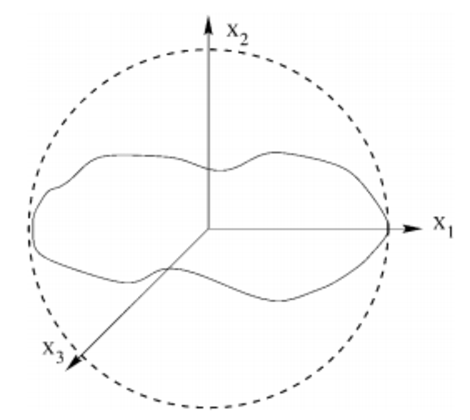
\includegraphics[width=\textwidth, height=0.25\textheight, keepaspectratio=true]{Brillouin_sphere.pdf}
\caption{Brillouin sphere or the circumscribing sphere around an irregular body \parencite{romain2001ellipsoidal}.}
\label{fig:brillouin_sphere}
\end{figure}
\FloatBarrier
%%%
Now consider a general statement for the gravity field of any arbitrary mass distribution $\mathcal{B}$ \parencite{scheeresBook}:
%%%
\begin{align}
    U = \frac{\mu}{V} \int_{\mathcal{B}} \frac{dV}{|\bvector{r} - \bvector{\rho}|}
    \label{eqn:general_gravity_field}
\end{align}
%%%
where $V$ is the volume, $\bvector{r}$ is the position vector to the point where the potential is being calculated, $\bvector{\rho}$ is the position vector to the discrete mass distribution within $\mathcal{B}$. If the potential is being calculated for a point that lies outside the maximum radius of the mass distribution being considered, then the integrand in \Cref{eqn:general_gravity_field} can be expanded into the following Laplace series form \parencite{scheeresBook}:
%%%
\begin{align}
    \frac{1}{|\bvector{r} - \bvector{\rho}|} = \frac{1}{r} \sum_{i=0}^{\infty} \left(\frac{\rho}{r}\right)^i P_{i0} \left(\frac{\bvector{r} \cdot \bvector{\rho}}{r\rho}\right)
    \label{eqn:general_grav_term_laplace_series}
\end{align}
%%%
where $P_{i0}$ are the Legendre polynomials. Thus using \Cref{eqn:general_grav_term_laplace_series}, the integral in \Cref{eqn:general_gravity_field} can be restated as follows \parencite{scheeresBook}:
%%%
\begin{align}
    \frac{\mu}{r} \cdot \left[ \frac{1}{V} \int_{\mathcal{B}} \left(\frac{\rho}{r}\right)^i P_{i0} \left(\frac{\bvector{r} \cdot \bvector{\rho}}{r\rho}\right) dV \right]
    \label{eqn:general_gravity_field_modified_integral}
\end{align}
%%%
There is a one-to-one correspondence between the term in the square brackets in \Cref{eqn:general_gravity_field_modified_integral} and the $i$th degree and order spherical harmonics gravity field. Thus by looking at the Laplace series in \Cref{eqn:general_grav_term_laplace_series} and the integral in \Cref{eqn:general_gravity_field_modified_integral}, we can infer on the convergence or divergence of the spherical harmonics gravity field. Since the maximum radius of the mass distribution in case of the spherical harmonics model would be that of the circumscribing or Brillouin sphere, then for a point on this sphere, i.e. $r = |\bvector{\rho}|$, the Laplace series is not defined and for a point inside the sphere, i.e. $r < |\bvector{\rho}|$, the Laplace series diverges. This is the limitation for using the spherical harmonics model for an irregular body when one wants to compute orbital motion in close proximity to the body. If the computation points are within the Brillouin sphere, the spherical harmonics series might diverge to a value that does not represent the true gravity potential value and hence lead to errors in orbit computations. We can see from \Cref{fig:brillouin_sphere} that the volume of divergence for irregularly shaped asteroids can be quite significant. Thus, this model is definitely not suitable for our research since we are dealing with close-proximity orbits and above all, particle re-impact scenarios.
%%%
\begin{figure}[htb]
\centering
\captionsetup{justification=centering}
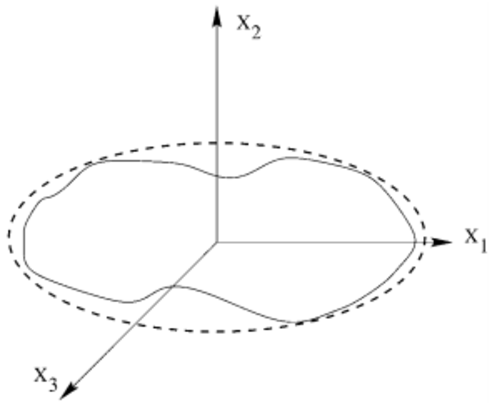
\includegraphics[width=\textwidth, height=0.25\textheight, keepaspectratio=true]{Brillouin_ellipsoid.pdf}
\caption{Brillouin ellipsoid or the circumscribing ellipsoid around an irregular body \parencite{romain2001ellipsoidal}.}
\label{fig:brillouin_ellipsoid}
\end{figure}
\FloatBarrier
%%%
The above problem can be mitigated, to a certain extent, by using the \textit{ellipsoidal harmonics} expansion for representing the gravity potential of an irregular body. An extremely detailed account on this model is given by \cite{dechambre2002transformation}. In the ellipsoidal harmonics model, instead of a sphere, a triaxial ellipsoid is used to circumscribe the irregular body and this proves to be a better fit as shown in \Cref{fig:brillouin_ellipsoid}. The ellipsoidal harmonics potential is given as follows \parencite{dechambre2002transformation}:
%%%
\begin{align}
    U(\lambda_1, \lambda_2, \lambda_3) &= \mu \sum_{n=0}^{\infty} \sum_{p=1}^{2n+1} \alpha_{np} \frac{E_n^p(\lambda_1)}{E_n^p(\lambda_1^{ref})} \times E_n^p(\lambda_2) E_n^p(\lambda_3) \text{; $\lambda_1 \leq \lambda_1^{ref}$}
    \label{eqn:ellipsoidal_harmonics_inside} \\
    U(\lambda_1, \lambda_2, \lambda_3) &= \mu \sum_{n=0}^{\infty} \sum_{p=1}^{2n+1} \alpha_{np} \frac{F_n^p(\lambda_1)}{F_n^p(\lambda_1^{ref})} \times E_n^p(\lambda_2) E_n^p(\lambda_3) \text{; $\lambda_1 \geq \lambda_1^{ref}$}
    \label{eqn:ellipsoidal_harmonics_outside}
\end{align}
%%%
where $(\lambda_1, \lambda_2, \lambda_3)$ are the ellipsoidal coordinates, which are basically three real roots (solutions) in terms of $s$ for the following conic equation \parencite{garmier2002modeling}:
%%%
\begin{align}
    \frac{x^2}{s^2 + a^2} + \frac{y^2}{s^2 + b^2} + \frac{z^2}{s^2 + c^2} = 1
    \label{eqn:conic_ellipsoidal}
\end{align}
%%%
where $(x, y, z)$ are the Cartesian coordinates and $(a, b, c)$ are the semi-axes of the reference ellipsoid circumscribing the irregular body (note that $a=\lambda_1^{ref}$). In \Cref{eqn:ellipsoidal_harmonics_inside,eqn:ellipsoidal_harmonics_outside}, $(\lambda_1, \lambda_2, \lambda_3)$ are analogous to the radius $r$, latitude $\delta$ and longitude $\lambda$, respectively, of \Cref{eqn:spherical_harmonics_general}; $\alpha_{np}$ is the ellipsoidal harmonics expansion coefficient similar to the spherical harmonics coefficient $C_{lm}$ and $S_{lm}$; $F_n^p()$ are the Lam\'e function of second kind of degree $n$ and order $p$ and is analogous to the attenuation term $(r_0 / r)^l$ of the spherical harmonics expansion in \Cref{eqn:spherical_harmonics_general}; $E_{n}^p()$ is the Lam\'e function of the first kind of degree $n$ and order $p$; and finally, the product term $E_{n}^p(\lambda_2)E_{n}^p(\lambda_3)$ is analogous to the product term $P_{lm} (\sin\delta) [C_{lm}\cos m\lambda + S_{lm}\sin m\lambda]$ which in both cases models the surface harmonic \parencite{garmier2002modeling}. A detailed description on definition and calculation of the ellipsoidal harmonic coefficients and the Lam\'e functions of the first and the second kind can be found in \cite{dechambre2002transformation} and is not repeated here for brevity.
%
\newline\newline
%
Even in the case of ellipsoidal harmonics expansion model, the gravity potential calculated for a point inside the circumscribing ellipsoid can diverge from the true potential. But the advantage of this model over the spherical harmonics expansion is that the circumscribing reference ellipsoid reduces the volume of divergence around the irregular body, relative to a sphere, making close-proximity evaluations possible. However, relative to the spherical harmonics expansion, the computation of the basis functions for ellipsoidal harmonics, i.e. the Lam\'e functions of the first and the second kind, is extremely complex. On top of that, with increasing degree of the harmonics model, the order of magnitude of the Lam\'e functions increases, which then runs the risk of arithmetic overflow, thereby impeding accurate calculations of the harmonic expansion for degrees above 10 to 15 \parencite{reimond2016spheroidal}. However, in their research, \cite{reimond2016spheroidal} have devised a new method to calculate the basis functions using logarithmic expressions which allows accurate harmonic expansions for degrees of upto 500 but the computational complexity also increases significantly as stated by them. Ultimately, since we wish to express the motion of particles close to the surface of the asteroid, which also involves surface interactions, the approach of ellipsoidal harmonics expansion also fails.

\section{Constant-Density Polyhedron}
\label{subsec:polyhedron}
The gravity potential modeling methods discussed so far involved the use of surface harmonics on the circumscribing object (sphere or ellipsoid) to simulate a non-homogeneous gravity field for an irregular body. The major drawback with the harmonics approach was its divergence from the true potential value within the circumscribing volume. This problem can be mitigated all together by assuming a specific shape and density distribution for the irregular body in question. In this realm, there are the \gls{CDE} and constant-density polyhedron gravity potential models. Unlike the harmonics expansion approach, these potential models are valid upto and on the surface of the shape that has been assumed for the irregular body in question \parencite{scheeresBook}. Hence, these models are perfect to study the close-proximity motion of particles or spacecraft around an asteroid.
%
\newline\newline
%
The irregular shape of an asteroid can be best represented by a polyhedron shape model (henceforth polyhedron) as shown in \Cref{fig:polyhedron_example}. Surface irregularities in the form of craters, large boulders, mountains etc. can be easily modeled with this method. A polyhedron is basically a 3D body that consists of several \textit{vertices} which form triangular faces or \textit{facets} that are connected to each other through the \textit{edges} of each face. A triangular facet thus comprises of three vertices, three edges and a surface normal as shown in \Cref{fig:single_facet} \parencite{scheeresBook}. A detailed derivation for the polyhedron gravity potential model is given in \cite{scheeres_polyhedra} and concisely presented in \cite{scheeresBook} as well. Hence, we will only present a summary of this method in this section.
%%%
\begin{figure}[htb]
\centering
\captionsetup{justification=centering}
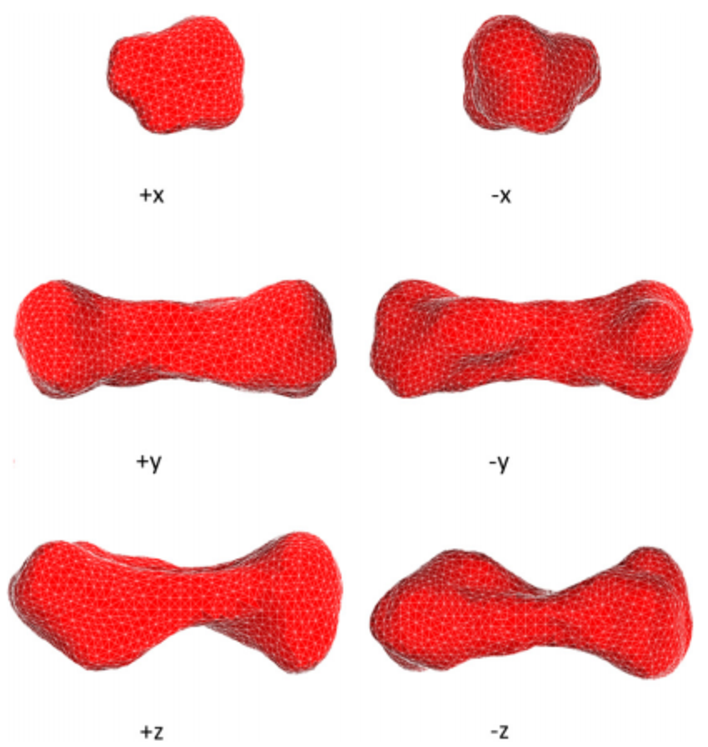
\includegraphics[width=\textwidth, height=0.3\textheight, keepaspectratio=true]{polyhedra_example.pdf}
\caption{Polyhedron shape model estimated for asteroid \textit{Kleopatra} and shown in $\pm x, \pm y, \pm z$ axis directions. Constant-density has been assumed. Surface irregularities are easily modeled by this method \parencite{polyhedra_example}.}
\label{fig:polyhedron_example}
\end{figure}
\FloatBarrier
%%%
%%%
\begin{figure}[htb]
\centering
\captionsetup{justification=centering}
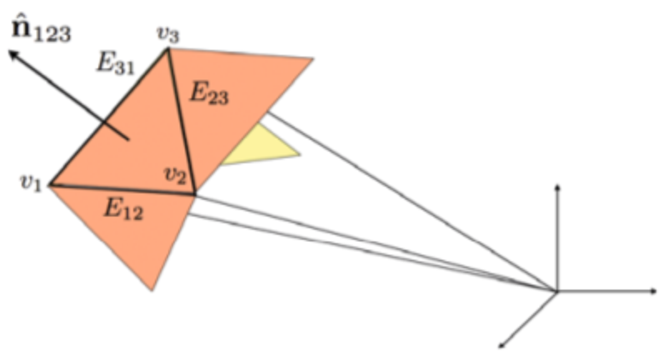
\includegraphics[width=\textwidth, height=0.2\textheight, keepaspectratio=true]{single_facet.pdf}
\caption{Single facet of a polyhedron model depicting three vertices, three edges and a surface normal, associated with each facet in general \parencite{scheeresBook}.}
\label{fig:single_facet}
\end{figure}
\FloatBarrier
%%%
Each face or facet \textit{'f'} of the polyhedron is associated with three vertex vectors given as $\bvector{r}_i^f$, where $i=1,2,3$, and a unit normal vector $\buvec{n}_f$. The vector $\bv{r}_i^f$ goes from each vertex of a facet to the field point \textbf{P} where the potential has to be calculated. Each edge \textit{'e'} is associated to two vertex vectors $\bvector{r}_i^e$, for $i=1,2$, and this edge connects two adjacent faces \textit{f} and \textit{f'}. Again, the vector $\bv{r}_i^e$ goes from the edge vertices to the field point \textbf{P}. The edge normal, corresponding to facet \textit{f}, is denoted as $\buvec{n}_e^f$ such that it is perpendicular to the edge and the facet normal $\buvec{n}_f$ and is pointing away from the centre of the facet. For the same edge shared by facet \textit{f'}, the edge normal $\buvec{n}_e^{f'}$ points in a different direction than $\buvec{n}_e^f$ and may not be parallel to it. With these definitions, the general formula for the polyhedron gravity potential is given as follows \parencite{scheeresBook}:
%%%
\begin{align}
    U(\bvector{r}) &= \frac{\mathcal{G}\sigma}{2} \left[ \sum_{e\in edges} \bvector{r}_e \cdotp \bm{E}_e \cdotp \bvector{r}_e L_e - \sum_{f\in faces} \bvector{r}_f \cdotp \bm{F}_f \cdotp \bvector{r}_f \omega_f \right]
    \label{eqn:polyhedron_potential} \\
    \bm{E}_e &= \buvec{n}_f \buvec{n}_e^f + \buvec{n}_{f'} \buvec{n}_e^{f'}
    \label{eqn:polyhedron_E_term} \\
    \bm{F}_f &= \buvec{n}_f \buvec{n}_f
    \label{eqn:polyhedron_F_term} \\
    L_e &= ln\left(\frac{r_1^e + r_2^e + e_e}{r_1^e + r_2^e - e_e} \right)
    \label{eqn:polyhedron_L_term} \\
    e_e &= |\bvector{r}_1^e - \bvector{r}_2^e|
    \label{eqn:polyhedron_e_term} \\
    \omega_f &= 2 \tan^{-1} \left(\frac{\bv{r}_1^f \cdotp (\bv{r}_2^f \times \bv{r}_3^f)}{r_1^f r_2^f r_3^f + r_1^f(\bv{r}_2^f \cdotp \bv{r}_3^f) + r_2^f(\bv{r}_3^f \cdotp \bv{r}_1^f) + r_3^f(\bv{r}_1^f \cdotp \bv{r}_2^f)} \right)
\end{align}
%%%
where \bvt{r} is the position vector to the field point \textbf{P} from the origin of an asteroid-fixed reference frame; $\mathcal{G}$ is the universal gravitational constant and $\sigma$ is the density of the body being modeled; $\bvector{r}_e$ is the vector from any point along the edge \textit{'e'} to \bvt{r} or the field point \textbf{P} and in the same way $\bvector{r}_f$ denotes a vector from any point on the facet \textit{f} to \bvt{r} \parencite{scheeresBook}; the term $\omega_f$ represents the solid angle subtended by a facet when viewed from the field point \textbf{P}, or alternately, it is the angle subtended by the facet of the polyhedron on to a unit sphere centered at the field point \textbf{P}; $L_e$ is analogous to the potential of a 1D straight \textit{'wire'} and is computed for all facet edges in a polyhedron \parencite{scheeres_polyhedra}; $\bm{E}_e$ is the edge dyad and is expressed as the sum of two outer products, forming a 3x3 matrix; and finally $\bm{F}_f$ is the facet dyad which is simply the outer product of the facet normal vector with itself \parencite{scheeres_polyhedra}.
%
\newline\newline
%
% The constant-density polyhedron gravity potential model provides a realistic shape for an irregular body by accounting for topographical irregularities; however, the model is computationally expensive \parencite{scheeresBook}. This thesis work does not make use of this model, but instead employs a triaxial ellipsoid to model the gravity potential (explained in the following section). This is because we want to understand the fundamental phenomena associated with the motion and final fate of regolith in the presence of gravity and Solar perturbations. This fundamental phenomena would be difficult to decouple from other effects of a true irregular body, such as in the case of a polyhedron model and hence it was not used in this thesis. A triaxial ellipsoid itself is a very good approximation of real small body shapes \parencite{broschart2005control} and hence we do not loose out on the validity of explanations for the fundamental features of regolith motion by excluding the polyhedron model.
